\documentclass{beamer}
%
% Choose how your presentation looks.
%
% For more themes, color themes and font themes, see:
% http://deic.uab.es/~iblanes/beamer_gallery/index_by_theme.html
%
\mode<presentation>
{
  \usetheme{Boadilla}      % or try Darmstadt, Madrid, Warsaw, ...
  \usecolortheme{beaver} % or try albatross, beaver, crane, ...
  \usefonttheme{default}  % or try serif, structurebold, ...
  \setbeamertemplate{navigation symbols}{}
  \setbeamertemplate{caption}[numbered]
  
} 

\usepackage{xcolor,colortbl}
\usepackage[english]{babel}
\usepackage[utf8x]{inputenc}
\usepackage{courier}
\usepackage{dsfont}
\usepackage{verbatim} 
\usepackage{enumerate}
\usepackage{tikz}
\usepackage{multirow}
\usepackage{venndiagram}
\usepackage{epigraph} 
%\usepackage{xcolor}
\usepackage{makecell}

%\usepackage{enumitem}

\usepackage{hyperref}
\hypersetup{
    colorlinks=true,
    linkcolor=blue,
    filecolor=magenta,      
    urlcolor=cyan,
}

% R stuff!
\usepackage{listings}
\definecolor{codegreen}{rgb}{0,0.6,0}
\definecolor{codegray}{rgb}{0.5,0.5,0.5}
\definecolor{codepurple}{rgb}{0.58,0,0.82}
\definecolor{backcolour}{rgb}{0.95,0.95,0.92}

\lstdefinestyle{mystyle}{
    backgroundcolor=\color{backcolour},    
    commentstyle=\color{codegreen},
    keywordstyle=\color{black},
    numberstyle=\tiny\color{codegray},
    stringstyle=\color{codepurple},
    basicstyle=\ttfamily\footnotesize,
    breakatwhitespace=false,         
    breaklines=true,                 
    captionpos=b,                    
    keepspaces=true,                 
    numbers=left,                    
    numbersep=5pt,                  
    showspaces=false,                
    showstringspaces=false,
    showtabs=false,                  
    tabsize=2
}

\lstset{style=mystyle}


\setbeamertemplate{enumerate items}[default]
\setbeamertemplate{itemize item}[triangle]

%\setitemize{label=\usebeamerfont*{itemize item}%
%  \usebeamercolor[fg]{itemize item}
%  \usebeamertemplate{itemize item}}



\title[Introduction to Statistics]{Probability Distributions}
\subtitle{}
\author{Grinnell College}
\date{}

\graphicspath{{img/}}

\begin{document}

\begin{frame}
  \titlepage
\end{frame}

%%%%%%%%%%%%%%%%%%%%%%%%%%%%%%%%%%%%%%%%%%%%%%%%%%%%%%%%%%%%%%%%
\begin{frame}{Normal Distribution}
\begin{center}
    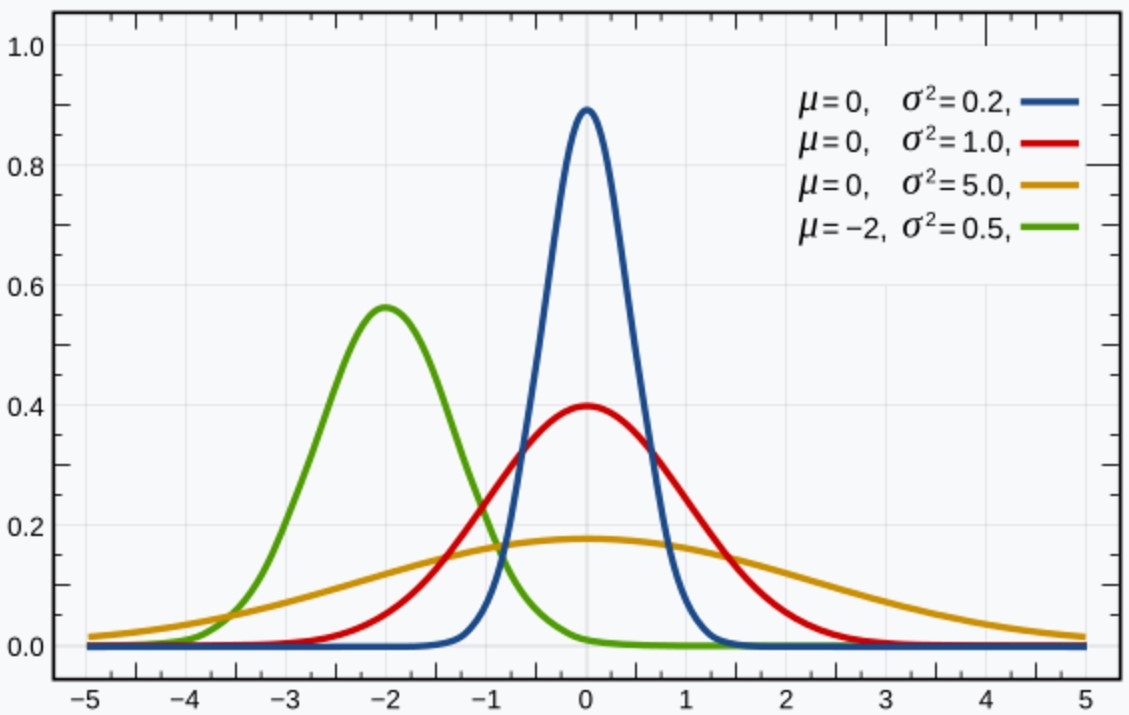
\includegraphics[scale=.4]{img/normaldist.jpg}
\end{center}
Distribution function: $f(x) = \frac{1}{\sqrt{2\pi}\sigma}e^{-\frac{(x-\mu)^2}{2\sigma^2}}$ \vspace{2mm}

This thing shows up \textit{everywhere}
\begin{itemize}
    \item population distributions
    \item sampling distributions for means and proportions
    \begin{itemize}
        \item CLT
    \end{itemize}
\end{itemize}
\end{frame}


%%%%%%%%%%%%%%%%%%%%%%%%%%%%%%%%%%%%%%%%%%%%%%%%%%%%%%%%%%%%%%%%
\begin{frame}{t-Distribution}
\begin{center}
    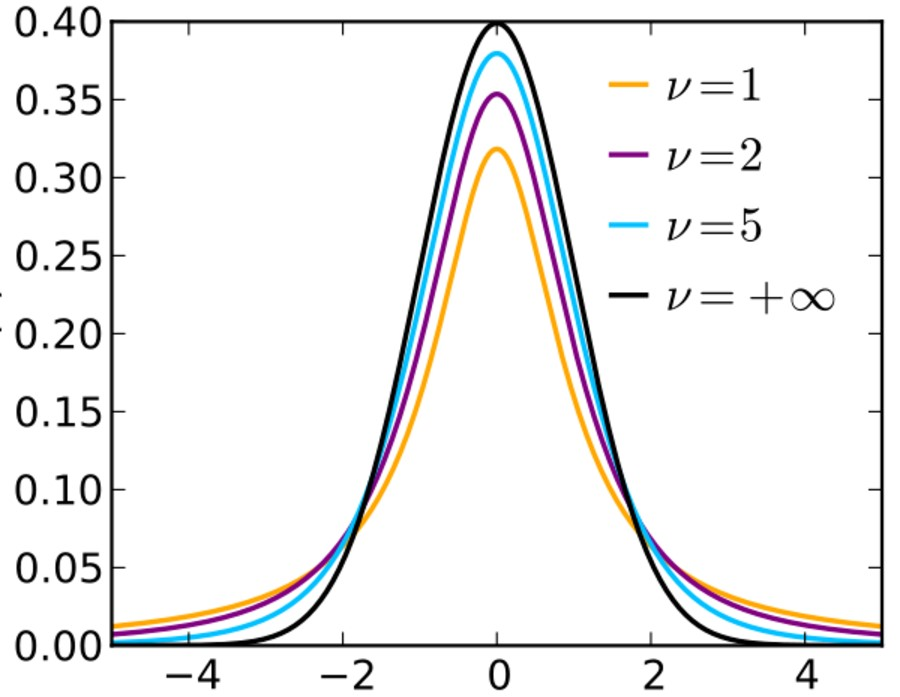
\includegraphics[scale=.35]{img/t-distribution.jpg}
\end{center}
Distribution function: $\frac{\Gamma\bigl(\frac{\nu+1}{2}\bigr)}{%
   \sqrt{\nu\pi}\,\Gamma\bigl(\frac{\nu}{2}\bigr)}
   \biggl(1+\frac{x^2}{\nu}\biggr)^{\!\!-(\frac{\nu+1}{2})}$, parameter: $\nu$ = df
\begin{itemize}
    \item $\mu = 0$, $\sigma^2 = \frac{\nu}{\nu-2}$ for $\nu > 2$, $\infty$ for $1 < \nu \leq 2$, otherwise undefined
    \item shows up when we standardize a Normal variable but don't know $\sigma$
    \item T test-statistic: T = $\frac{\overline{x}-\mu}{s / \sqrt{n}} \sim t_{n-1}$
\end{itemize}
\end{frame}

%%%%%%%%%%%%%%%%%%%%%%%%%%%%%%%%%%%%%%%%%%%%%%%%%%%%%%%%%%%%%%%%
\begin{frame}{$\chi^2$-Distribution ("kai"-squared)}
\begin{center}
    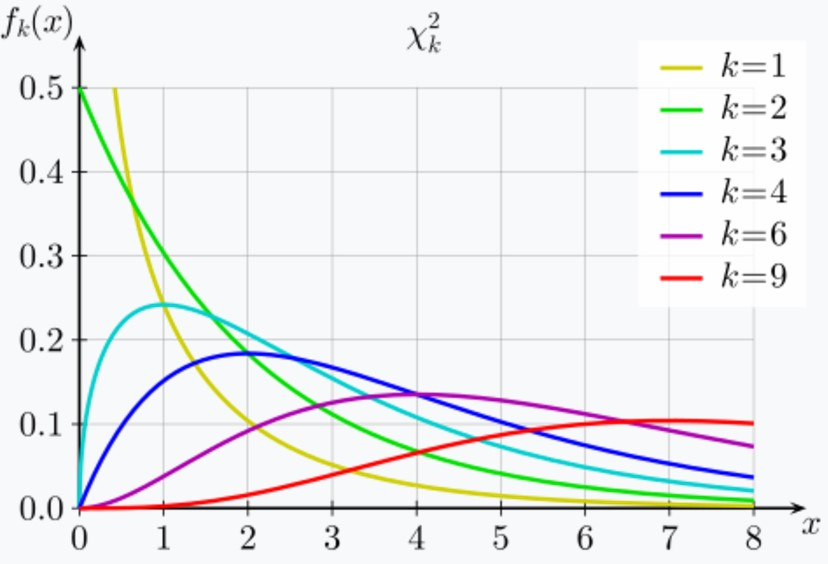
\includegraphics[scale=.45]{img/chi2_distr.jpg}
\end{center}

\begin{itemize}
    \item $\mu = k$, $\sigma^2 = 2k$
    \item only parameter is k = df = degrees of freedom
\end{itemize}
\end{frame}


%%%%%%%%%%%%%%%%%%%%%%%%%%%%%%%%%%%%%%%%%%%%%%%%%%%%%%%%%%%%%%%%
\begin{frame}{$\chi^2$-Distribution}
\begin{center}
    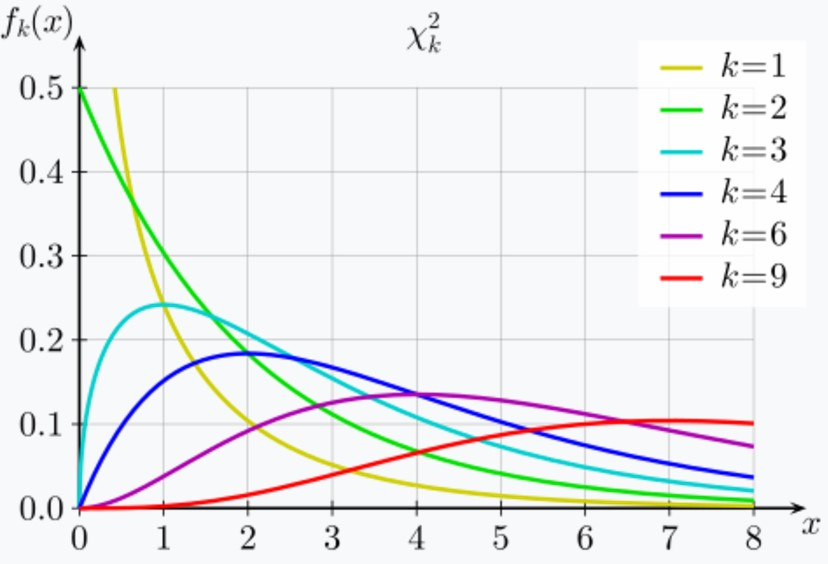
\includegraphics[scale=.3]{img/chi2_distr.jpg}
\end{center}
Ok, but where does this distribution come from? \vspace{4mm}

Suppose I have a whole bunch of Standard Normal variables $X_1, X_2, ... , X_k$ that are all independent (not influencing each other)
\begin{itemize}
    \item If I square and add them, I get something that has a $\chi^2$ distribution
    \item df = (k-1) where k is the number of Normals I used
\end{itemize} \vspace{4mm}
\begin{center}
$\sum_{i=1}^k X_i^2 \sim \chi^2_{k-1}$
\end{center}
\end{frame}

%%%%%%%%%%%%%%%%%%%%%%%%%%%%%%%%%%%%%%%%%%%%%%%%%%%%%%%%%%%%%%%%
\begin{frame}{$\chi^2$-Distribution}
$Z = \frac{\overline{x}-\mu}{\sigma / \sqrt{n}} \sim N(0,1) \rightarrow Z^2 \sim \chi^2_{0}$ \hspace{2mm} \textbf{ISSUE:} can't have k=0 (only 1 group)
\begin{itemize}
    \item $\chi^2$ only works for more than 1 group (differences)
\end{itemize}\vspace{8mm}

Could have done this:

$Z_1 = \frac{\overline{x}_1-\mu_1}{\sigma_1 / \sqrt{n}_1} \sim N(0,1)$

$Z_2 = \frac{\overline{x}_2-\mu_2}{\sigma_2 / \sqrt{n}_2} \sim N(0,1)$

$Z_1^2 + Z_2^2 = (\frac{\overline{x}_1-\mu_1}{\sigma_1 / \sqrt{n}_1})^2 + (\frac{\overline{x}_2-\mu_2}{\sigma_2 / \sqrt{n}_2})^2 \sim \chi^2_1$
\begin{itemize}
    \item could have used this distribution to talk about diff. in means
    \item but... Normal distribution is easier
    \item this \textbf{does} come in more handy for differences in proportions
\end{itemize}
\end{frame}

\begin{frame}{$\chi^2$ Hypothesis Tests}

The most common forms of hypotheses we will be testing with the $\chi^2$-test:

\begin{align*}
    H_0: p_1 = p_2 \textbf{ OR } H_0: p_1 - p_2 = 0\\
    H_A: p_1 \neq p_2 \textbf{ OR } H_A: p_1 - p_2 \neq 0
\end{align*}
\vspace{3mm}

If we have N $>$ 2 groups
\begin{align*}
    H_0: p_1 = ... p_N \textbf{ OR } H_0: \text{all proportions are the same}\\
    H_A: \text{at least one proportion is different than the others}
\end{align*} \vspace{3mm}

Pro's and Con's:
\begin{itemize}
    \item $\chi^2$-tests work for any number of groups
    \item only works for '$\neq$' hypotheses
\end{itemize}
\end{frame}

\begin{frame}{$\chi^2$ Hypothesis Tests}
A bit more general -- we can test if all the proportions are equal to different specified values, but writing the general hypothesis forms get complicated.
\begin{itemize}
    \item there is no agreed on notation for this I am aware of, usually specified qualitatively with context
\end{itemize}
\begin{align*}
    H_0: p_1 = p_{1_{(o)}}, p_2 = p_{2_{(o)}}, ..., p_N = p_{N_{(o)}}\\
    \textbf{ OR } H_0: \text{all proportions equal the specified value}
\end{align*}
\begin{align*}
    H_A: \text{at least one proportion is different than the specified value}
\end{align*}
\end{frame}


\begin{frame}{Problem}
The 'final' exam is coming up. Suppose (hypothetically), that I am lazy and want to write an exam that is particularly easy to grade, so I make 5 questions that are true/false. But, also suppose (hypothetically) that I am mean and make the questions incredibly difficult. \vspace{6mm}

Given that there are 26 students in this class, I can look through the results and make the following table to compare how many people got a question right (Observed) and compare that to how many I would expect to get the question right by guessing (Expected).
\vspace{6mm}

% latex table generated in R 4.4.2 by xtable 1.8-4 package
% Tue Nov 19 15:47:57 2024
\begin{table}[ht]
\centering
\begin{tabular}{rrrrrr}
  \hline
Question & 1 & 2 & 3 & 4 & 5 \\ 
  \hline
Expected & 13 & 13 & 13 & 13 & 13 \\ 
  Observed & 10 & 14 & 15 & 11 & 9 \\ 
   \hline
\end{tabular}
\end{table}
\end{frame}

\begin{frame}{Goodness of Fit}

The $\chi^2$ (chi squared or ``kai" squared) \textbf{goodness of fit} test allows us to compared \textit{expected} proportions in $k$ groups against those we \textit{observe}
\begin{align*}
\chi^2 &= \sum_{i=1}^k \frac{(\text{Expected}_i - \text{Observed}_i)^2}{\text{Expected}_i} 
\end{align*}
Under the null hypothesis (equality of proportions to 'expected' proportions), for $k$ groups, the $\chi^2$ goodness of fit test statistic follows a $\chi^2$ distribution with $k-1$ degrees of freedom
\begin{align*}
\chi^2 \sim \chi^2(k-1)
\end{align*}

\end{frame}

\begin{frame}
% latex table generated in R 4.4.2 by xtable 1.8-4 package
% Tue Nov 19 15:47:57 2024
\begin{table}[ht]
\centering
\begin{tabular}{rrrrrr}
  \hline
Question & 1 & 2 & 3 & 4 & 5 \\ 
  \hline
Expected & 13 & 13 & 13 & 13 & 13 \\ 
  Observed & 10 & 14 & 15 & 11 & 9 \\  
   \hline
\end{tabular}
\end{table}

\begin{align*}
\chi^2 &= \sum_{i=1}^k \frac{(\text{Expected}_i - \text{Observed}_i)^2}{\text{Expected}_i} \\[1em]
&= \frac{(10-13)^2}{13} + \frac{(14-13)^2}{13} + \frac{(15-13)^2}{13} + \frac{(11-13)^2}{13}+\frac{(9-13)^2}{13} \\[1em]
&= \frac{9 + 1 + 4 + 4 + 16}{13} \approx 2.62
\end{align*}

\end{frame}

\begin{frame}{Samples}

\begin{table}[ht]
\centering
\begin{tabular}{rrrrrr}
  \hline
 & A & B & C & D & E \\ 
  \hline
Sample 1 &  14 &  14 &  11 &  11 &  15 \\ 
  Sample 2 &  13 &  13 &  14 &  11 &  14 \\ 
  Sample 3 &  15 &  15 &  15 &  13 &   7 \\ 
  Sample 4 &  12 &  15 &  10 &  15 &  13 \\ 
  Sample 5 &  13 &  16 &  10 &   7 &  19 \\ 
  Sample 6 &  15 &  11 &  17 &   8 &  14 \\ 
  Sample 7 &  10 &  10 &  14 &  16 &  15 \\ 
  Sample 8 &   7 &  17 &  14 &  12 &  15 \\ 
  Sample 9 &  15 &   5 &  13 &  14 &  18 \\ 
  Sample 10 &  13 &  15 &  17 &  14 &   6 \\ 
   \hline
\end{tabular}
\end{table}

\end{frame}

\begin{frame}{Samples}
\begin{table}[ht]
\centering
\begin{tabular}{rrrrrrr}
  \hline
 & A & B & C & D & E & chi \\ 
  \hline
Sample 1 & 14 & 14 & 11 & 11 & 15 & 1.08 \\ 
  Sample 2 & 13 & 13 & 14 & 11 & 14 & 0.46 \\ 
  Sample 3 & 15 & 15 & 15 & 13 & 7 & 3.69 \\ 
  Sample 4 & 12 & 15 & 10 & 15 & 13 & 1.38 \\ 
  Sample 5 & 13 & 16 & 10 & 7 & 19 & 6.92 \\ 
  Sample 6 & 15 & 11 & 17 & 8 & 14 & 3.85 \\ 
  Sample 7 & 10 & 10 & 14 & 16 & 15 & 2.46 \\ 
  Sample 8 & 7 & 17 & 14 & 12 & 15 & 4.46 \\ 
  Sample 9 & 15 & 5 & 13 & 14 & 18 & 7.23 \\ 
  Sample 10 & 13 & 15 & 17 & 14 & 6 & 5.38 \\ 
   \hline
\end{tabular}
\end{table}

\end{frame}


\begin{frame}
\begin{center}
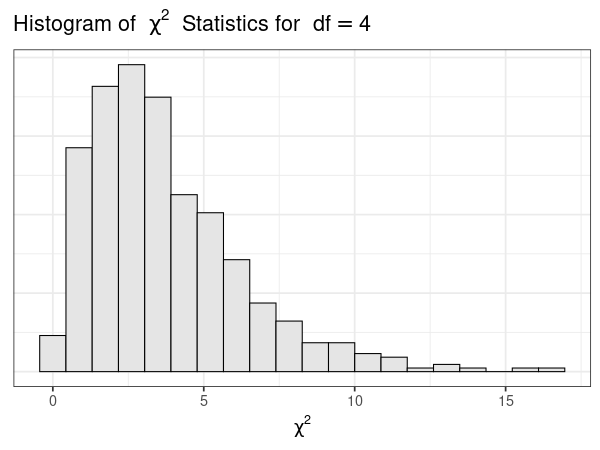
\includegraphics[scale=0.5]{chisq_hist.png}
\end{center}
\end{frame}

\begin{frame}
\begin{center}
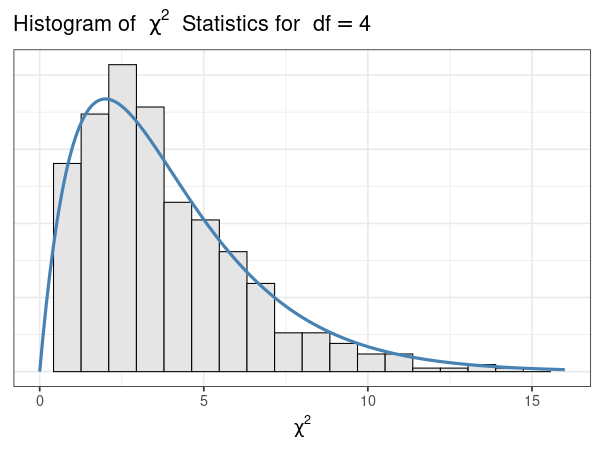
\includegraphics[scale=0.5]{chisq_hist2.png}
\end{center}
\end{frame}

\begin{frame}{$p$-value for exam questions}
\begin{center}
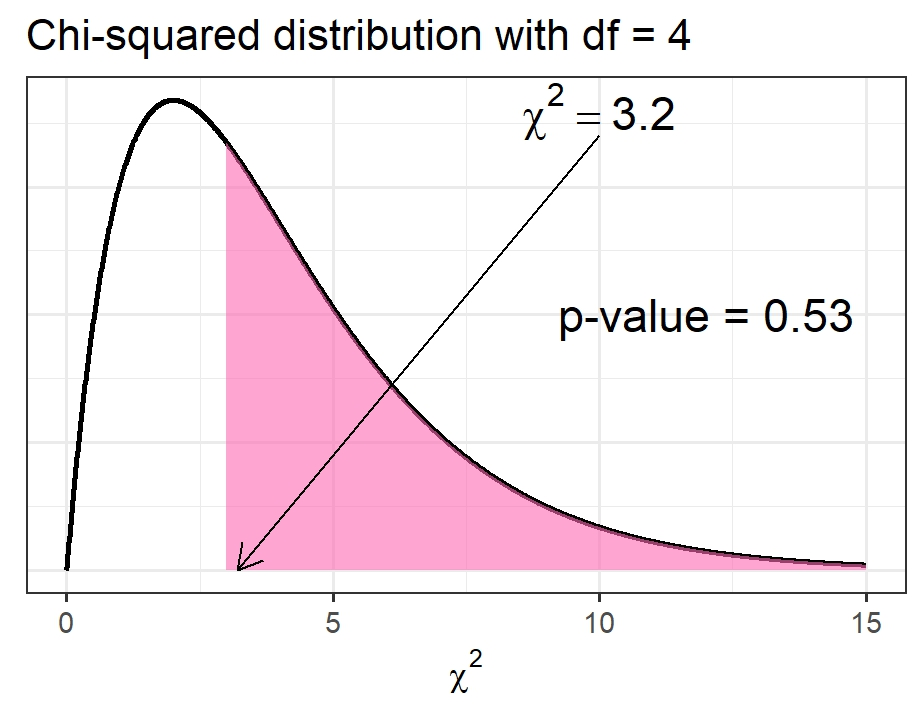
\includegraphics[scale=0.65]{img/chisq_p.jpeg}
\end{center}
\end{frame}


\begin{frame}
\begin{center}
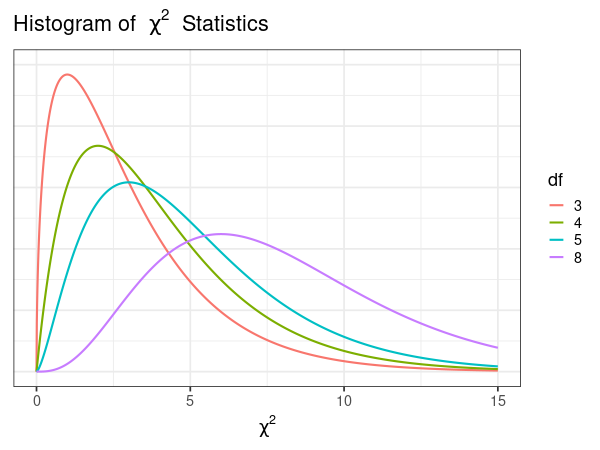
\includegraphics[scale=0.5]{chisq.png}
\end{center}
\end{frame}

\begin{frame}{$p$-value for $\chi^2$}
\begin{align*}
\chi^2 &= \sum_{i=1}^k \frac{(\text{Expected}_i - \text{Observed}_i)^2}{\text{Expected}_i} 
\end{align*}
A few things to note about this statistic:
\begin{itemize}
\item It's always positive (or equal to zero)
\item The more our observed values deviate from our expected, the larger it gets
\end{itemize}
From this, we get two facts:
\begin{itemize}
\item Our $p$-value is computed as the area \textit{to the right} of our test statistic
\item Greater values of $\chi^2$ indicate more evidence against the null hypothesis
\end{itemize}
\end{frame}


\begin{frame}{Jury Example}
Prospective jurors are supposed to be randomly chosen from the eligible adults in a community. The American Civil Liberties Union (ACLU) studied the racial composition of the jury pools in 10 trials in Alameda County, California. Display below is the racial and ethnicity composition of the $n = 1,453$ individuals included in the jury pools, along with the distribution of eligible jurors according to US Census data: \vspace{3mm} 
\footnotesize
% latex table generated in R 4.3.3 by xtable 1.8-4 package
%% Wed Apr 17 11:37:06 2024
\begin{table}[ht]
\centering
\begin{tabular}{rrrrrrr}
  \hline
Race Ethnicity & White & Black & Hispanic & Asian & Other & Total \\ 
  \hline
Jury Size & 780 & 117 & 114 & 384 & 58 & 1453 \\
Census Percentage & 54\% & 18\% & 12\% & 15\% & 1\% & 100\% \\
   \hline
\end{tabular}
\end{table}
\end{frame}

\begin{frame}{Jury Example -- R code}
\begin{table}[ht]
\centering
\begin{tabular}{rrrrrrr}
  \hline
Race Ethnicity & White & Black & Hispanic & Asian & Other & Total \\ 
  \hline
Jury Size & 780 & 117 & 114 & 384 & 58 & 1453 \\
Census Percentage & 54\% & 18\% & 12\% & 15\% & 1\% & 100\% \\
   \hline
\end{tabular}
\end{table}

\begin{center}
    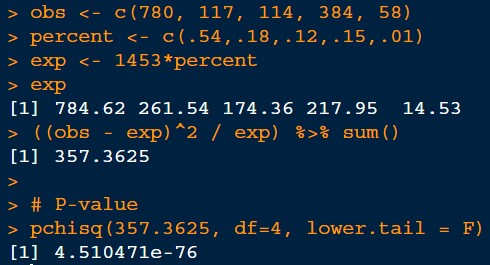
\includegraphics[scale=1]{img/juryexample_rcode.jpg}
\end{center}
\end{frame}

%%%%%%%%%%%%%%%%

%\begin{frame}
%\begin{columns}
%
%  \begin{column}{0.45\textwidth}
%%
%  \end{column}
%  \begin{column}{0.45\textwidth}
%%
%  \end{column}
%
%\end{columns}
%\end{frame}


\end{document}


